% !TEX TS-program = pdflatex
% !TEX encoding = UTF-8 Unicode

% This is a simple template for a LaTeX document using the "article" class.
% See "book", "report", "letter" for other types of document.

%commento
\documentclass[11pt]{article} % use larger type; default would be 10pt

\usepackage[utf8]{inputenc} % set input encoding (not needed with XeLaTeX)

%%% PAGE DIMENSIONS
\usepackage{geometry} % to change the page dimensions

\geometry{a4paper} % or letterpaper (US) or a5paper or....
% \geometry{margin=2in} % for example, change the margins to 2 inches all round
% \geometry{landscape} % set up the page for landscape
%   read geometry.pdf for detailed page layout information

\usepackage{caption}
\usepackage{subcaption}
\usepackage{graphicx, xcolor} % support the \includegraphics command and options

% \usepackage[parfill]{parskip} % Activate to begin paragraphs with an empty line rather than an indent

%%% PACKAGES
\usepackage{booktabs} % for much better looking tables
\usepackage{array} % for better arrays (eg matrices) in maths
\usepackage{paralist} % very flexible & customisable lists (eg. enumerate/itemize, etc.)
\usepackage{verbatim} % adds environment for commenting out blocks of text & for better verbatim
%\usepackage{subfig} % make it possible to include more than one captioned figure/table in a single float
% These packages are all incorporated in the memoir class to one degree or another...
\usepackage{genealogytree}
\gtruselibrary{all}

\usepackage{wrapfig}

\usepackage{nameref}

\usepackage[backend=bibtex]{biblatex}
\bibliography{bibliography.bib}

%%% HEADERS & FOOTERS
\usepackage{fancyhdr} % This should be set AFTER setting up the page geometry
\pagestyle{fancy} % options: empty , plain , fancy
\renewcommand{\headrulewidth}{0pt} % customise the layout...
\lhead{}\chead{}\rhead{}
\lfoot{}\cfoot{\thepage}\rfoot{}

%%% SECTION TITLE APPEARANCE
\usepackage{sectsty}
\allsectionsfont{\sffamily\mdseries\upshape} % (See the fntguide.pdf for font help)
% (This matches ConTeXt defaults)
\usepackage{pdfpages}
\usepackage{hyperref}
\hypersetup{
  colorlinks=true,%activates colors
  allcolors=blue,%default color
  linkcolor=blue,
  filecolor=magenta,      
  urlcolor=cyan,
}
  
%%% ToC (table of contents) APPEARANCE
\usepackage[nottoc,notlof,notlot]{tocbibind} % Put the bibliography in the ToC
\usepackage[titles,subfigure]{tocloft} % Alter the style of the Table of Contents
\renewcommand{\cftsecfont}{\rmfamily\mdseries\upshape}
\renewcommand{\cftsecpagefont}{\rmfamily\mdseries\upshape} % No bold!

%%% END Article customizations

%%% The "real" document content comes below...
%
\title{Memory effect in news' spreading networks: data analysis}
\author{Roberto Bertilone, Francesco Fanchin, Nicola Sella}
%\date{} % Activate to display a given date or no date (if empty),
         % otherwise the current date is printed 
\begin{document}

\maketitle

\newpage

\tableofcontents

\newpage

\section{Introduction}
Rumour spreading is a well-known phenomena in human interactions: its influence on public opinion and political elections is studied with different methodologies, derived from sociology, mathematics, physics, psicology and computer science.
DK model, (citazione), introduced by Dailey and Kendall, was one of the first attempts to mathematically reproduce the phenomena by stochastic differential equations: a famous variant is MK model.
With the development of complex networks, other approaches included network topology 
and different stochastic models like mean-field (cite) and interacting markov-chains (IMC)(cite).
Thanks to the rapid increasement in computing power, massive computer simulations have been made possible in most research and industry sectors.\\
Agent-based models (ABM) is a class of computational models for simulating the actions and interactions of autonomous agents.
Rumour spreading, in an ABM context, can be viewed as a network of interacting agents: from rules on single agent's behaviour,  a computer simulation will show the effects on the overall system.
This paper represents natural prosecution of the previous work,
''Memory effects in news' spreading networks'' by the same authors.\\
While the former described network's structure and agents' actions, this one clarifies the role of agents' memory length in network topology and news' distribution.
In the first section the focus will be on two network properties, average clustering coefficient and diameter.
In the second section we will point out the relation between memory size
and Gini index, to take into account inequalities within new's distribution. 
The whole model lacks, for the moment, of a validation with real data.

Does memory size have something connected with other properties?
we belive yes and we are expecting to find some correlations related
to information, spreading and entropy. Thus the use of Gini.\\ \\
Does a phenomenological approach make sense? \hl{Yes because abm needs
this type of approach (vedi slides)}\\ \\
Is this model validated with real data? \hl{Not yet.}
\hl{explain bubbles with image}

\newpage

\section{Data Analysis}
lhvlhvlhv.hj

\newpage

\section{Activation Time}
alsivbalsjvbasògjbòsgjòskj

\newpage

All agents in our network have a fixed \textit{memory length}, i.e. they can remember a maximum
 amount of news.
In this section, its influence in network topology will be studied: clustering and
 diameter are standard measures in network science's literarure and widely used to describe 
 network properties.\\
  Each of them will be plotted 
 against memory length to search possible correlations.
\subsection{Clustering} \label{clustering}
A large number of networks show a tendency for link formation between neighboring vertices, 
i.e., the network topology deviates from uncorrelated random networks: this tendency is called 
\textit{clustering} \cite{clusterarticle}. \\
For unweighted graphs, the clustering of a node $u$ is the fraction of possible triangles over 
all possible triplets  through that node that exist \cite{clustersite},

\begin{equation}
\label{eq:clustering}
c_u = \frac{2 T(u)}{deg(u)(deg(u)-1)}
\end{equation}
where $T(u)$ is the number of triangles through node $u$ and $deg(u)$ is the degree of $u$.
Hence, the \textit{average clustering coefficient}  is:
\begin{equation}
\label{eq:average_clustering}
ACC = \frac{1}{n}\sum_{v \in G} c_v
\end{equation}
We ask wether memory, previously considered in section \ref{introduction}, could affect the 
average clustering coefficient.
To answer the question, the following experiment was designed:
for every memory size, five simulations were run over a thousand iterations; $ACC$'s mean and 
standard deviation were computed afterwards.\\
Finally, via weighted interpolation, a plot of $ACC$'s mean over memory size will show possible
 correlations. \hl{Results and discussion are reported together with diameter}.
\begin{figure}[h]
  \centering
  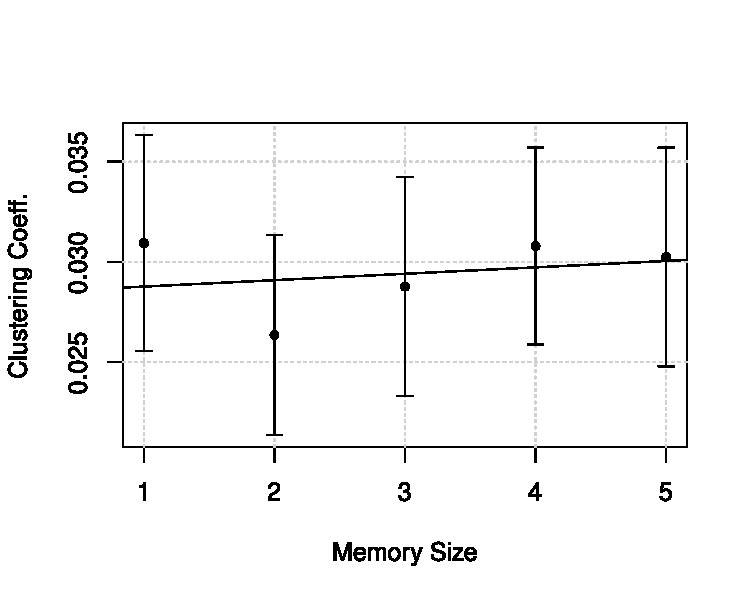
\includegraphics[trim={0cm 0cm 0cm 1cm},clip,width=.8\columnwidth]{img/clustering.pdf}
  \caption{$ACC$'s mean-memory size linear weighted fit: five simulations per point.}
  \label{fig:clustering}
\end{figure}


\newpage

\section{Diameter}
kjhflh,jhv,jg

\newpage

\section{Conclusion and further developments}
This paper has shown a correlation between memory length and Gini
index of news' distribution: a suitable optimization function
was developed in order to properly fit experimental data.
With reference to network topology, memory does not significantly
affect clustering and diameter.
There is not, at the moment, a clear evidence of echo chambers.\\
\\
Further developments include longer simulations with more nodes:
the overall system is not generally scale-invariant.
Hence, we expect different behaviors (like a more
distinct observation
of echo chambers) at higher orders of magnitude.\\
The presence of a phase transition in news' distribution could be investigated: in particular, the research should focus on its distinctive traits (critical exponents, order parameters...). 
In addition, other agents' actions or news' features could be added for a better realism.
For example, news are characterized by a certain amount of different topics.\\
However, they are not perceived as bad or good by agents: this additional ``degree of freedom''
could be inserted in the algorithm.




\end{document}